\documentclass[11pt]{article}
\usepackage[margin=.75in]{geometry}
\usepackage{amsmath,amssymb,graphicx,hyperref}
\setlength{\parindent}{0pt}\setlength{\parskip}{5pt}
\begin{document}
\begin{center}{\Large Actual weighted elliptic relation to a target scalar}\\27 November 2026 --- unsigned local Lean component evidence\end{center}
\textbf{Derived scalar.}
Given the actual principal factorization and exact nonsingular rational residual
point product, retain independent labels \(m_i\) for every non-target input
and \(r_j\) for every residual factor. Put
\[
 c=\sum_{i\ne t} n_i m_i+\sum_j r_j.
\]
Lean derives \(n_tQ+cP=0\). Under explicit \(\ell Q=0\) and
\(\gcd(n_t,\ell)=1\), the public extended-gcd identity constructs
\[
 Q=\bigl(-\operatorname{gcdA}(n_t,\ell)c\bigr)P.
\]
For actual generator order \(\ell\) and \(Q=kP\), the unknown \(k\) equals
that integer label modulo \(\ell\) (PCC-20261127-2c4548) [pcc:unverified].
\begin{center}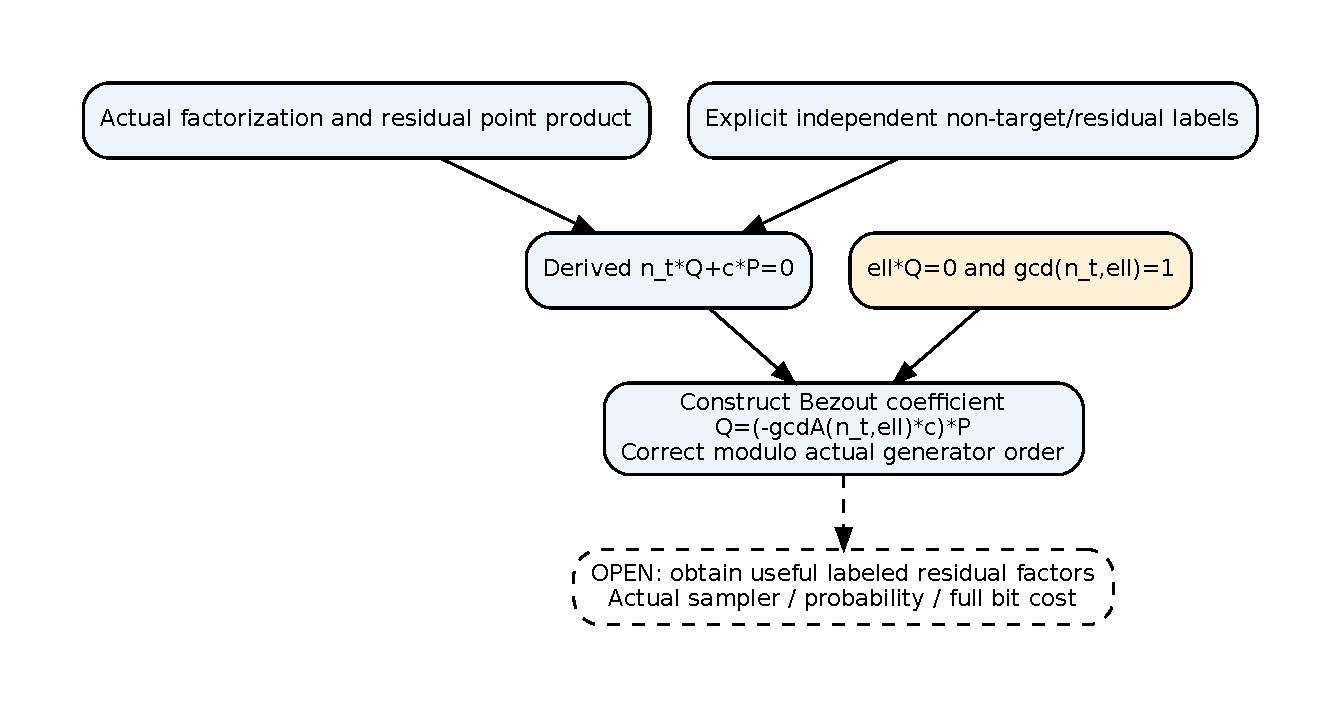
\includegraphics[height=2.65in,width=.97\linewidth,keepaspectratio]{weighted-scalar-dependencies-001.pdf}\end{center}
\textbf{Proof map.}
Namespace \texttt{OrientationActualWeightedScalar}, source100/build106/local053:
\begin{center}\begin{tabular}{ll}
\texttt{known\_weighted\_sum}&aggregate independently labeled inputs\\
\texttt{weighted\_label\_relation}&derive \(n_tQ+cP=0\)\\
\texttt{recover\_from\_coprime\_coefficient}&construct Bezout label\\
\texttt{recovered\_scalar\_modEq}&actual-order congruence\\
\texttt{actual\_target\_scalar}&compose actual point-ideal relation
\end{tabular}\end{center}
All263 printed statements (five new) have standard printed foundations;
exit zero, zero warnings and366 exact input bindings checked.
Candidate099/build105 exited zero with two tactic-sequence warnings and
was not accepted. Its source/raw output remain exact;100 changed only the
unnecessary sequence operator, with no linter suppression [pcc:unverified].

\textbf{Scope and next obligation.}
No residual label is supplied by the extraction proof itself, and no target
label is an input to its actual extraction theorem. Integer representatives
need not be canonical. The torsion and coprimality conditions are explicit.
Standard group and Bezout arithmetic is reused without novelty claims.
No gcd/normalization or complete preparation/bit runtime is inferred.
Next: an actual per-instance public procedure obtaining useful labeled
residual factors, with class-conditioned sampling success, retries and full
cost; no reusable-precomputation shortcut.

\textbf{Sources.}
Actual NormGroupBridge target extraction and accepted weighted residual
relation; public Mathlib integer congruence/order scalar laws and Nat extended
gcd. KB unavailable, exact source fallback used. Evidence is unsigned local,
outside historical shared Transport53/57 audit/fresh. Protocol019 and
continuation029 retain the next action.
\end{document}
